\documentclass{standalone}
\usepackage{tikz,tikz-qtree}
\usepackage[T1]{fontenc}
\begin{document}
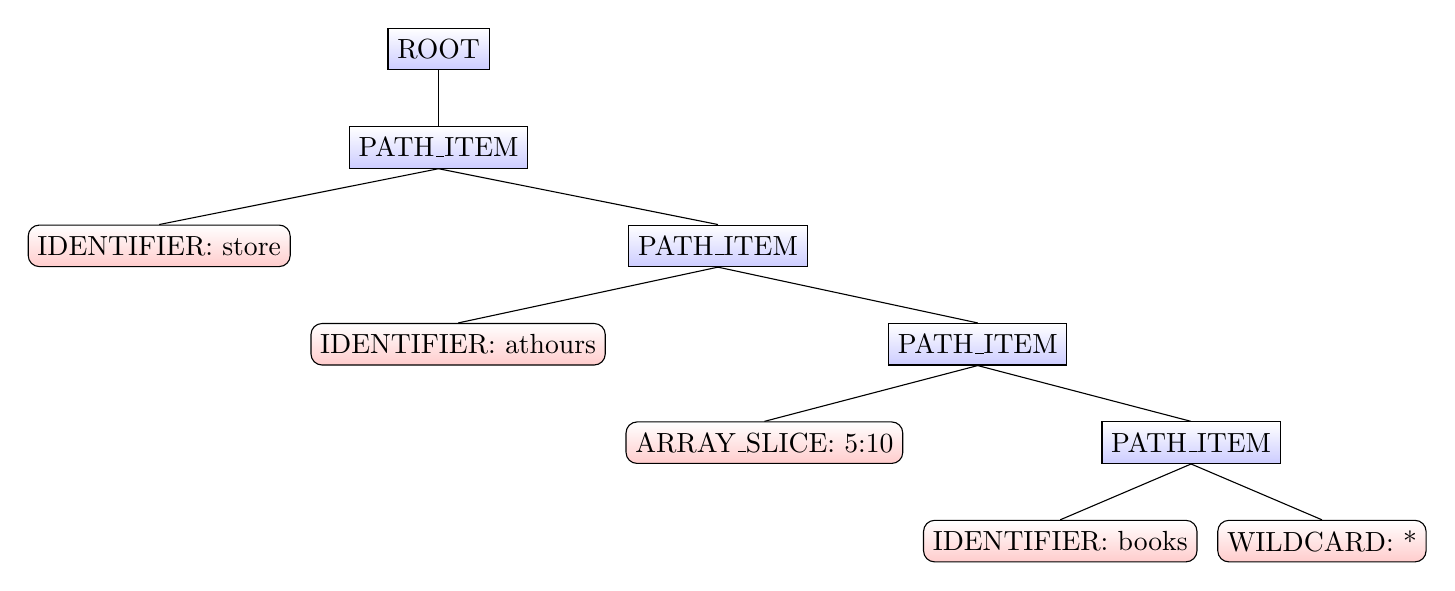
\begin{tikzpicture}
[level distance=1.25cm,sibling distance=.25cm,every tree node/.style={anchor=north,align=center,draw,top color=white, bottom color=blue!20,minimum width=1.5em,minimum height=1.5em},every leaf node/.style={anchor=north,align=center,draw,rounded corners,top color=white, bottom color=red!20,minimum width=1.5em,minimum height=1.5em},blank/.style={draw=none,color=white!0, top color=white!0, bottom color=white!0},]
\Tree
[.\node(0x5e700b0fbaf0){ROOT};
	[.\node(0x5e700b0fba80){PATH\_ITEM};
		\node(0x5e700b0fb430){ IDENTIFIER: store};
		[.\node(0x5e700b0fba10){PATH\_ITEM};
			\node(0x5e700b0fb510){ IDENTIFIER: athours};
			[.\node(0x5e700b0fb9a0){PATH\_ITEM};
				\node(0x5e700b0fb6c0){ ARRAY\_SLICE: 5:10};
				[.\node(0x5e700b0fb930){PATH\_ITEM};
					\node(0x5e700b0fb7d0){ IDENTIFIER: books};
					\node(0x5e700b0fb8e0){WILDCARD: *};
				]
			]
		]
	]
]
\end{tikzpicture}
\end{document}
